\documentclass[12pt]{article}
\usepackage{amsmath}
\usepackage{pgfplots}
\usepackage{tikz}
\pgfplotsset{compat = 1.18}
\title{\textbf{Option 1: driving fuel efficiency}}
\author{Eric Zhou}
\begin{document}

\maketitle

\begin{equation*}
    E(v) = \frac{80v}{v^2 + 20}
\end{equation*}

%\begin{tikzpicture}
%\draw[blue, domain = -2:2, smooth] plot (\x, {80 * \x / (\x * \x + 20)});
%\end{tikzpicture}

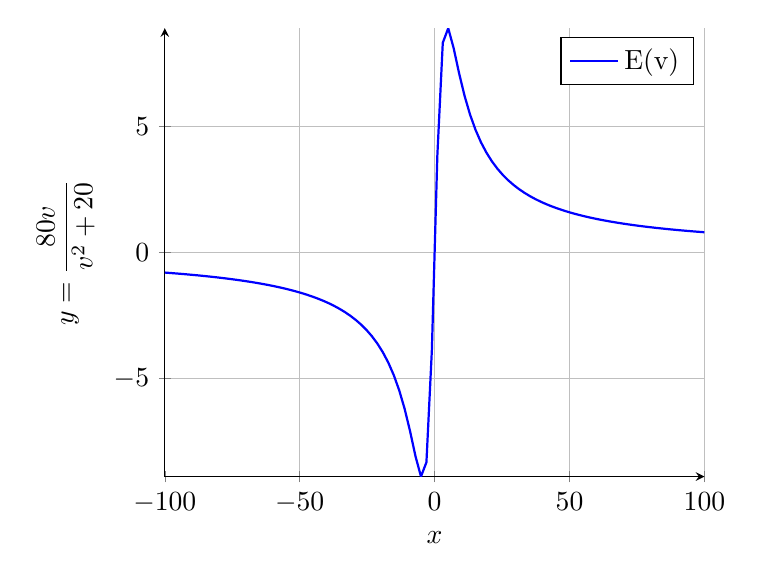
\begin{tikzpicture}
    \centering
    \begin{axis}[
        axis lines = left,
        xlabel = \(x\),
        ylabel = {\(y = \dfrac{80 v} {v^2 + 20}\)},
        grid = both,
        domain = -100:100, % Range for x
        samples = 100, % Smoothness
    ]
    \addplot[color=blue, thick] {{80 * x / (x * x + 20)}}; % Function to plot
    \legend{E(v)} % Optional legend
    \end{axis}
\end{tikzpicture}

\section{Modeling}

As the speed increases, the fuel efficiency first increases and then reduces.

Since

\begin{equation*}
    \begin{aligned}
        & \lim_{v\rightarrow +\infty} E(x)  \\
       =& \lim_{v\rightarrow +\infty} \frac{80v}{v^2 + 20} \\
       =& \lim_{v\rightarrow +\infty} \frac{80}{2v} \\
       =& 0 \\
    \end{aligned}
\end{equation*}

The horizontal asymptote is $y = 0$. It means as the speed increases, the efficiency decreases and gets infinitely close to zero but never reaches zero.

%\section*{Derivative of \( E(v) = \frac{80v}{v^2 + 20} \)}
\section{Optimization}

The optimal driving strategy should be maximizing the efficiency. To find the maximum of a continuous function, we can try find the zeros of its derivative.

The quotient rule can be applied for differentiation:
\begin{equation*}
\left( \frac{a}{b} \right)' = \frac{a'b - ab'}{b^2}
\end{equation*}
where $ a = 80v $ and $ b = v^2 + 20 $.

The differentiation of $a$ and $b$ is trivial

\begin{equation*}
\begin{aligned}
a &= 80v \quad \Rightarrow \quad a' = 80, \\
b &= v^2 + 20 \quad \Rightarrow \quad b' = 2v.
\end{aligned}
\end{equation*}

Therefore

\begin{equation*}
\begin{aligned}
    E'(v) &= \frac{a'b - ab'}{b^2} = \frac{(80)(v^2 + 20) - (80v)(2v)}{(v^2 + 20)^2} \\
    E'(v) &= \boxed{\frac{-80(v^2 - 20)}{(v^2 + 20)^2}}.
\end{aligned}
\end{equation*}

$E'(v)$ is zero only when $v^2 - 20$ is zero. $v = \pm\sqrt{20} = \pm{2\sqrt{5}}$. The negative one does not make sense in the real circumstance. Therefore $E(v)$ reaches its maximum when $v = 2\sqrt{5} \approx 4.47$.

\end{document}